% !TEX TS-program = XeLaTeX
% !TEX encoding = UTF-8 Unicode

\chapter{图表及公式的格式说明}
\label{chap02}
\defaultfont
\section{图的格式说明}
\subsection{图的格式示例}
图在正文中的格式示例如图2.1所示。
\begin{figure}
	\centering
	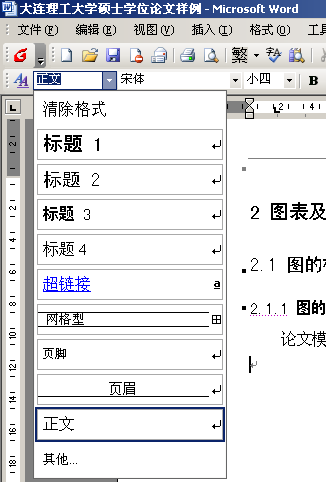
\includegraphics[scale = 0.4]{figures/2.1}
	\caption{\song\wuhao 样式}
\end{figure}

表、图序号后面,同样适当留空(汉字状态敲两次空格键)。

图2.1显示了论文模板中所定义的样式选择方法。使用鼠标选择相应的样式,对应的文字格式就发生相应改变。

\subsection{图的格式描述}
(1) 图的绘制方法
\begin{enumerate}[label=\circled{\arabic*}]
\item 插图、照片应尽量通过扫描粘贴进本文。
\item 简单文字图可用WORD直接绘制,复杂的图考虑使用相应的图形绘制软件完成,提高图形表达质量。
\end{enumerate}

(2) 图的位置
\begin{enumerate}[label=\circled{\arabic*}]
\item 图居中排列。
\item 图与上文之间应留一空行。
\item 图中若有附注,一律用阿拉伯数字和右半圆括号按顺序编排,如注1),附注写在图的下方。
\end{enumerate}

(3) 图的版式
\begin{enumerate}[label=\circled{\arabic*}]
\item “设置图片格式”的“版式”为“上下型”或“嵌入型”,不得“浮于文字之上”。
\item 图的大小尽量以一页的页面为限,不要超限,一旦超限要加续图。
\item 图中若有附注,一律用阿拉伯数字和右半圆括号按顺序编排,如注1),附注写在图的下方。
\end{enumerate}

(4) 图名的写法
\begin{enumerate}[label=\circled{\arabic*}]
\item 图名居中并位于图下,编号应分章编号,如图2.1。
\item 图名与下文留一空行。
\item 图及其名称要放在同一页中,不能跨接两页。
\item 图内文字清晰、美观。
\item 图名设置为宋体,五号,居中。
\end{enumerate}

\section{表的格式说明}
\subsection{表的格式示例}
表在正文中的常用格式如表2.1至表2.3所示,请参考使用。

物流的概念和范围如表2.1表述。

表、图序号与后面文字同样应当适当留空(两次空格键)。

\begin{table}
	\centering
	\song\wuhao 
	\caption{物流的概念和范围}
	\begin{tabular}{cc}
	\hline
	本质&过程\\
	\hline
	途径或方法&规划、实施、控制\\
	目标&效率、成本效益\\
	活动或作业&流动与存储\\
	处理对象&原材料、在制品、产成品、相关信息\\
	范围&从原点(供应商)到终点(最终顾客)\\
	目的或目标&适应顾客的需求(产品、功能、数量、质量、时间、价格)\\
	\hline
	\end{tabular}
\end{table}

美国广义物流后(勤)协会给出的定义如下:“为了符合顾客的要求,从原点到消费点对原材料、在制品、产成品与相关信息的流动和储存的效率成本效益进行规划、实施和控制的过程”。由此可见,物流不是作为一种具体技术和方法来研究的,而是一个过程或管理。

\begin{table}
	\centering
	\song\wuhao
	\caption{ 统计表}
	\begin{tabular}{ccccc}
	\hline
	年度&产量&销量&产值&比重\\
	\hline
	手机&11000&10000&500&50\%\\
	电视机&5500&5000&220&22\%\\
	计算机&1100&1000&280&28\%\\
	\hline
	合计&17600&16000&1000&100\%\\
	\hline
	\end{tabular}
\end{table}

\begin{table}
	\centering
	\song\wuhao
	\caption{ 分栏表}
	\begin{tabular}{ccccc}
	\hline
	年度&产品&产量&销量&产值\\
	\hline
	2004&手机&11000&10000&500\%\\
	2004&计算机&1100&1000&280\%\\
	\hline
	2005&手机&16000&13000&550\%\\
	2005&计算机&2100&1500&320\%\\
	\hline
	\end{tabular}
\end{table}

从表2.2和表2.3可以看出,公司销售情况。

\subsection{表的格式描述}
(1) 表的绘制方法

表要用WORD绘制,不要粘贴。

(2) 表的位置
\begin{enumerate}[label=\circled{\arabic*}]
\item 表格居中排列。
\item 表格与下文应留一行空格。
\item 表中若有附注,一律用阿拉伯数字和右半圆括号按顺序编排,如注1),附注写在表的下方。
\end{enumerate}

(3) 表的版式
\begin{enumerate}[label=\circled{\arabic*}]
\item 表的大小尽量以一页的页面为限,不要超限,一旦超限要加续表。
\end{enumerate}

(4) 表名的写法
\begin{enumerate}[label=\circled{\arabic*}]
\item 表名应当在表的上方并且居中。编号应分章编号,如表2.1、表2.2。
\item 表名与上文留一空行
\item 表及其名称要放在同一页中,不能跨接两页。
\item 表内文字全文统一,设置为宋体,五号。
\item 表名设置为宋体,五号,且居中。
\end{enumerate}

\section{公式的格式说明}
\subsection{公式的格式示例}
由于一般的文献资料中所给出的载荷和抗力的统计参数主要为变异系数,为便于讨论,定义公式形式如下:
\begin{equation}
LRI = 1/\sqrt{1+(\frac{\mu_R}{\mu_s})^2(\frac{\delta_R}{\delta_S})^2}
\end{equation}
其中,$\mu_R$和$\mu_S$分别为抗力和载荷效应的均值,……。

\subsection{公式的格式描述}
(1) 公式整行右对齐,并调整公式与公式序号之间的距离,使公式部分居中显示。

(2) 公式序号应按章编号,公式编号在行末列出,如(2.1)、(2.2)。

(3) 公式位置:公式之间及上下文间设置半行间距或者6磅,作者可根据情况适当调整,以保证格式协调和美观。

\section{参考文献的格式说明}
\subsection{参考文献在正文中的引用实例}
关于主题法的起源众说不一。国内有人认为“主题法检索体系的形式和发展开始于1856年英国克雷斯塔多罗(Crestadoro)的《图书馆编制目录技术》一书”,“国外最早采用主题法来组织目录索引的是杜威十进分类法的相关主题索引……”。也有人认出为“美国的贝加逊·富兰克林出借图书馆第一个使用了主题法”。

\subsection{参考文献在正文中引用的书写格式}
引用的文献在正文中用方括号和阿拉伯数字按顺序以右上角标形式标注在引用处。

\subsection{参考文献的书写格式}
(1) 参考文献按照在正文中引用的顺序进行编码。

(2) 作者一律姓前名后(外文作者名应缩写),作者间用“,”间隔。作者少于3人应全部写出,3人以上只列出前3人,后加“等”或“et al”。

(3) 标题“参考文献”选用模板中的样式所定义的“参考文献”,再居中;或者手动设置成字体:黑体,居中,字号:小三,1.5倍行距,段后1行,段前为0行。

(4) 参考文献正文设置成字体:宋体,居左,字号:五号,多倍行距1.25行,段后、段前均为0行。

(5) 按照引用的文献类型不同使用不同的表示方法。
\begin{enumerate}[label=\circled{\arabic*}]
\item 专著(注意应标明出版地及所参阅内容在原文献中的位置),表示方法为:

[序号] 作者.专著名[文献类型标志].出版地:出版者,出版年.
\item 期刊中析出的文献(注明应标明年、卷、期,尤其注意区分卷和期号),表示方法为:

[序号] 作者.题(篇)名[文献类型标志].刊名.出版年,卷号(期号):起止页.
\item 会议论文,表示方法为:

[序号] 作者.篇名[文献类型标志].会议名,会址,开会年: 起止页.
\item 专著(文集)中析出的文献,表示方法为:

[序号] 作者.篇名[文献类型标志].见(In):文集的编(著)者.文集名.出版地:出版者,出版年:起止页.
\item 学位论文,表示方法为:

[序号] 作者.题(篇)名[文献类型标志]:(博(硕)士学位论文).授学位地:授学位单位,授学位年.
\item 学位论文,表示方法为:

[序号] 专利申请者.专利题名[文献类型标志].专利国别,专利文献种类,专利号.出版日期.
\end{enumerate}

\subsection{参考文献的书写格式示例}
文献类型标志及参考文献书写示例请见“参考文献”部分。

\section{量和单位的使用}
\subsection{使用方法}
\begin{enumerate}
\item 必须符合国家标准规定,不得使用已废弃的单位,如高斯(G和Gg)﹑亩﹑克分子浓度(M)﹑当量能度(N)等。
\item 量和单位不用中文名称,而用法定符号表示。
\end{enumerate}

\subsection{中华人名共和国法定计量单位}
中华人民共和国法定计量单位如表2.4至表2.8所示。
\begin{table}
	\centering
	\song\wuhao
	\caption{国际单位制的辅助单位}
	\begin{tabular}{ccc}
	\hline
	量的名称&单位名称&单位符号\\
	\hline
	平面角&弧度&rad\\
	立体角&球面度&sr\\
	\hline
	\end{tabular}
\end{table}

\begin{table}
	\centering
	\song\wuhao
	\caption{国际单位制中具有专门名称的导出单位}
	\begin{tabular}{cccc}
	\hline
	量的名称&单位名称&单位符号&其它表示示例\\
	\hline
	频率&赫[兹]&Hz&$s^{-1}$\\
	力;重力&牛[顿]&N&$kg·m/s^2$\\
	压力,压强;应力&帕[斯卡]&Pa&$N/m^2$\\
	能量;功;热&焦[耳]&J&$N/m$\\
	功率;辐射通量&瓦[特]&W&$J/s$\\
	电荷量&库[仑]&C&$A.s$\\
	电位;电压;电动势&伏[特]&V&$W/A$\\
	电容&法[拉]&F&$C/V$\\
	电阻&欧[姆]&$\Omega$&$V/A$\\
	电导&西[门子]&S&$A/V$\\
	磁通量&韦[伯]&Wb&$V.S$\\
	磁通量密度,磁感应强度&特[斯拉]&T&$Wb/m^2$\\
	电感&亨[利]&H&$Wb/A$\\
	摄氏温度&摄氏度&$^\circ$C&~\\
	光通量&流明&lm&$cd·sr$\\
	光照度&勒[克斯]&lx&$lm/m^2$\\
	放射性活度&贝可[勒尔]&Bq&$s^{-1}$\\
	吸收剂量&戈[瑞]&Gy&$J/kg$\\
	剂量当量&希[沃特]&Sv&$J/kg$\\
	\hline
	剂量当量&希[沃特]&Sv&$J/kg$\\
	\hline
	\end{tabular}
\end{table}

\begin{table}
	\centering
	\song\wuhao
	\caption{国际单位制的基本单位}
	\begin{tabular}{ccc}
	\hline
	量的名称&单位名称&单位符号\\
	\hline
	长度&米&m\\
	质量&千克(公斤)&kg\\
	时间&秒&s\\
	电流&安[培]&A\\
	热力学温度&开[尔文]&K\\
	物质的量&摩[尔]&mol\\
	发光强度&坎[德拉]&cd\\
	\hline
	\end{tabular}
\end{table}

\begin{table}
	\centering
	\song\wuhao
	\caption{国家选定的非国际单位制单位}
	\begin{tabular}{cccc}
	\hline
	量的名称&单位名称&单位符号&换算关系和说明\\
	\hline
	时间&分&min&1min=60s\\
	时间&[小]时&h&1h=60min=3600s\\
	时间&天(日)&d&1d=24h=86400s\\
	旋转速度&转每分&r/min&$1r/min=(1/60)s^{-1}$\\
	长度&海里&n mile&1n mile = 1852m\\
	速度&节&Kn&=(1852/3600)m/s\\
	质量&吨&t&$1t=10^3kg$\\
	体积&升&L&$1L=1dm3=10^{-3}m^3$\\
	能&电子伏&eV&$1eV=1.6021892*10^{-19}J$\\
	级差&分贝&db&~\\
	超密度&特[克斯]&tex&1 tex=1g/km\\
	\hline
	\end{tabular}
\end{table}

\begin{table}
	\centering
	\song\wuhao
	\caption{用于构成十进倍数和分数单位的词头}
	\begin{tabular}{ccc}
	\hline
	所表示的因数&词头名称&词头符号\\
	\hline
	$10^{18}$&艾[克萨]&E\\
	$10^{15}$&拍[它]&P\\
	$10^{12}$&太[拉]&T\\
	$10^{9}$&吉[咖]&G\\
	$10^{6}$&兆&M\\
	$10^{3}$&千&K\\
	$10^{2}$&百&h\\
	$10^{1}$&十&da\\
	$10^{-1}$&分&d\\
	$10^{-2}$&厘&c\\
	$10^{-3}$&毫&m\\
	$10^{-6}$&微&$\mu$\\
	$10^{-9}$&纳[诺]&n\\
	$10^{-12}$&皮[可]&p\\
	$10^{-15}$&飞[母托&a\\
	$10^{-18}$&阿[托]&a\\
	\hline
	\end{tabular}
\end{table}

\section{规范表达注意事项}
\subsection{名词术语}
应使用全国自然科学名词审定委员会审定的自然科学名词术语;应按有关的标准或规定使用工程技术名词术语;应使用公认共知的尚无标准或规定的名词术语。作者自拟的名词术语,在文中第一次出现时,须加注说明。表示同一概念或概念组合的名词术语,全文中要前后一致。外国人名可使用原文,不必译出。一般的机关、团体、学校、研究机构和企业等的名称,在论文中第一次出现时必须写全称。

\subsection{数字}
数字的使用必须符合新的国家标准GB/T15835-1995《出版物上数字用法的规定》。

\subsection{外文字母}
文中出现的易混淆的字母、符号以及上下标等,必须打印清楚或缮写工整。要严格区分外文字母的文种、大小写、正斜体和黑白体等,必要时用铅笔注明,尤其注意上下标字母的大小写、正斜体。

(1) 斜体

斜体外文字母用于表示量的符号,主要用于下列场合:

\begin{enumerate}[label=\circled{\arabic*}]
\item 变量符号、变动附标及函数。
\item 用字母表示的数及代表点、线、面、体和图形的字母。
\item 特征数符号,如Re(雷诺数)、Fo(傅里叶数)、Al(阿尔芬数)等。
\item 在特定场合中视为常数的参数
\item 矢量、矩阵用黑体斜体。
\end{enumerate}

(2) 正体

正体外文字母用于表示名称及与其有关的代号,主要用于下列场合:

\begin{enumerate}[label=\circled{\arabic*}]
\item 有定义的已知函数(例如$\sin$,$\exp$,$\ln$等)。
\item 其值不变的数学常数(例如$e=2.718 281 8…$)及已定义的算子。
\item 法定计量单位、词头和量纲符号。。
\item 数学符号
\item 化学元素符号。
\item 机具、仪器、设备和产品等的型号、代号及材料牌号。
\item 硬度符号。
\item 不表示量的外文缩写字。
\item 表示序号的拉丁字母。
\item 量符号中为区别其它量而加的具有特定含义的非量符号下角标。
\end{enumerate}

\subsection{量和单位}
文中涉及的量和单位一律采用新的国家标准GB3100~3102-93《量和单位》。

\subsection{标点符号}
标点符号的使用必须符合新的国家标准GB/T15834-1995《标点符号用法》。
